\subsubsection{Tomadas - Generalidades}\label{section: socket-general}

\begin{enumerate}
		
	\item Em caso de \textit{retrofit} de ambientes, pavimentos ou edificações, o número de tomadas a serem projetadas \textbf{não} podem ser dimensionadas em quantidade inferior as quantidades levantadas em campo.
	
	\item Nos casos de \textit{retrofit} em ambientes, pavimentos ou edificações cujo \textit{layout} existente seja modificado, o projetista deverá considerar no mínimo as tomadas dos equipamentos existentes no textit{layout} novo mais um adicional de tomadas (127 e 220V) na ordem de 20\% a mais em relação as quantidade de tomadas para os equipamentos existentes no layout.
	
	\item \label{socket: bitola minima} Em circuitos de tomadas, será adotado a bitola mínima de 4,0mm\textsuperscript{2}.
	
	\item \label{socket: bitola minima ar} Em circuitos de tomadas de ar-condicionado e estufas, será adotado a bitola mínima de 6,0mm\textsuperscript{2}.
	
	\item Não serão admitidas tomadas de 10A a exceção das tomadas preconizadas na seção \ref*{section: iluminacao_interiores} item \ref*{light:encaixe10A}
	
	\item Devem ser projetadas em todos os ambientes, tomadas 2P + T de 20A.
	
	\item Em estações de trabalho individualizado, devem ser previstas no mínimo 3(três) tomadas 127V/200W para cada estação de trabalho.
	
	\item Em laboratórios, salas de freezers ou ambientes congêneres deverá ser considerada a utilização de tomadas 127 e 220V.
	
	\item Em ambientes administrativos ou de ensino deverá ser considerada no mínimo a proporção de 1 tomada 220V para cada 3 ou 4 tomadas 127V (a critério do projetista e de acordo com as potências dos equipamentos)
	
	\item Não será aceita a utilização de eletrodutos de bitola menor que 1” de diâmetro para circuitos de tomadas.
	
	\item Poderá ser considerada a instalação como previsão de reserva, eletrodutos com bitolas superiores às necessárias para as bitolas iniciais dos condutores ou eletrodutos vazios.
	
	\item As tomadas de uso geral não poderão ser conectadas a circuitos de iluminação, à exceção das preconizadas na subseção \ref{section: iluminacao_interiores} itens \ref*{light:wc1} e \ref*{light:wc2}
	 
	\item Tomadas de uso específico deverão ser alimentadas através de circuitos individuais
	
	\item O projetista deverá dispor da forma mais uniforme possível, as tomadas nas paredes, nos rodapés ou no piso, observadas as eventuais particularidades decorrentes das condições construtivas do local e da ocupação a que se destinam.

	\item Tomadas para conectar geladeiras/freezers comuns poderão ser dispostas em até 4(tomadas) num mesmo circuito desde que as potências individuais não exceda 300W;
	
	\item Tomadas para conectar freezers com características especiais (temperaturas inferiores a 30 graus negativos) deverão ser alocados em circuitos individualizados;

	\item Para as tomadas, deverá ser adotada a bitola mínima de 4,0mm2 observando, entretanto, a diferenciação de cores nas respectivas fiações, inclusive nas redes estabilizadas e não-estabilizadas.

	\item Na especificação e cadernos de encargos ao ser confeccionado, distinguir tomadas 127V, 220V e 380V(se for o caso) e estabilizadas e não estabilizadas através do uso de cores das tampas de acabamento (quando avaliável).
	
	\item Caso existam no projeto, tomadas com tensão de 380V indicar graficamente 380V, sendo necessário constar em nota que as mesmas devem ser etiquetadas com "380V" quando executadas.
	
	\item Deve ser evitada utilização de tomadas de piso em todo o projeto, em casos excepcionais a contratante deverá ser consultada;
	
	\item Devido as características do padrão de tomadas brasileiro, indicar em projeto e na lista de materiais que as caixas conduletes / caixas de luz deverão ser adequadas para diâmetros de eletrodutos de 1”, e que as mesmas deverão ser acomodas com relativa folga;
	
	\item As tomadas deverão ser montadas em caixas conduletes(aparente) ou caixas de luz(embutidas) que permitam a instalação de eletrodutos de diâmetro mínimo de1”;
	
	\item As tomadas 127V deverão ser projetadas preferencialmente na cor branca ou bege
	
	\item As tomadas 220V deverão ser projetadas na cor vermelha;
	
		\begin{figure}[H]
			\centering
			\begin{subfigure}[b]{0.23\textwidth}
				\centering
				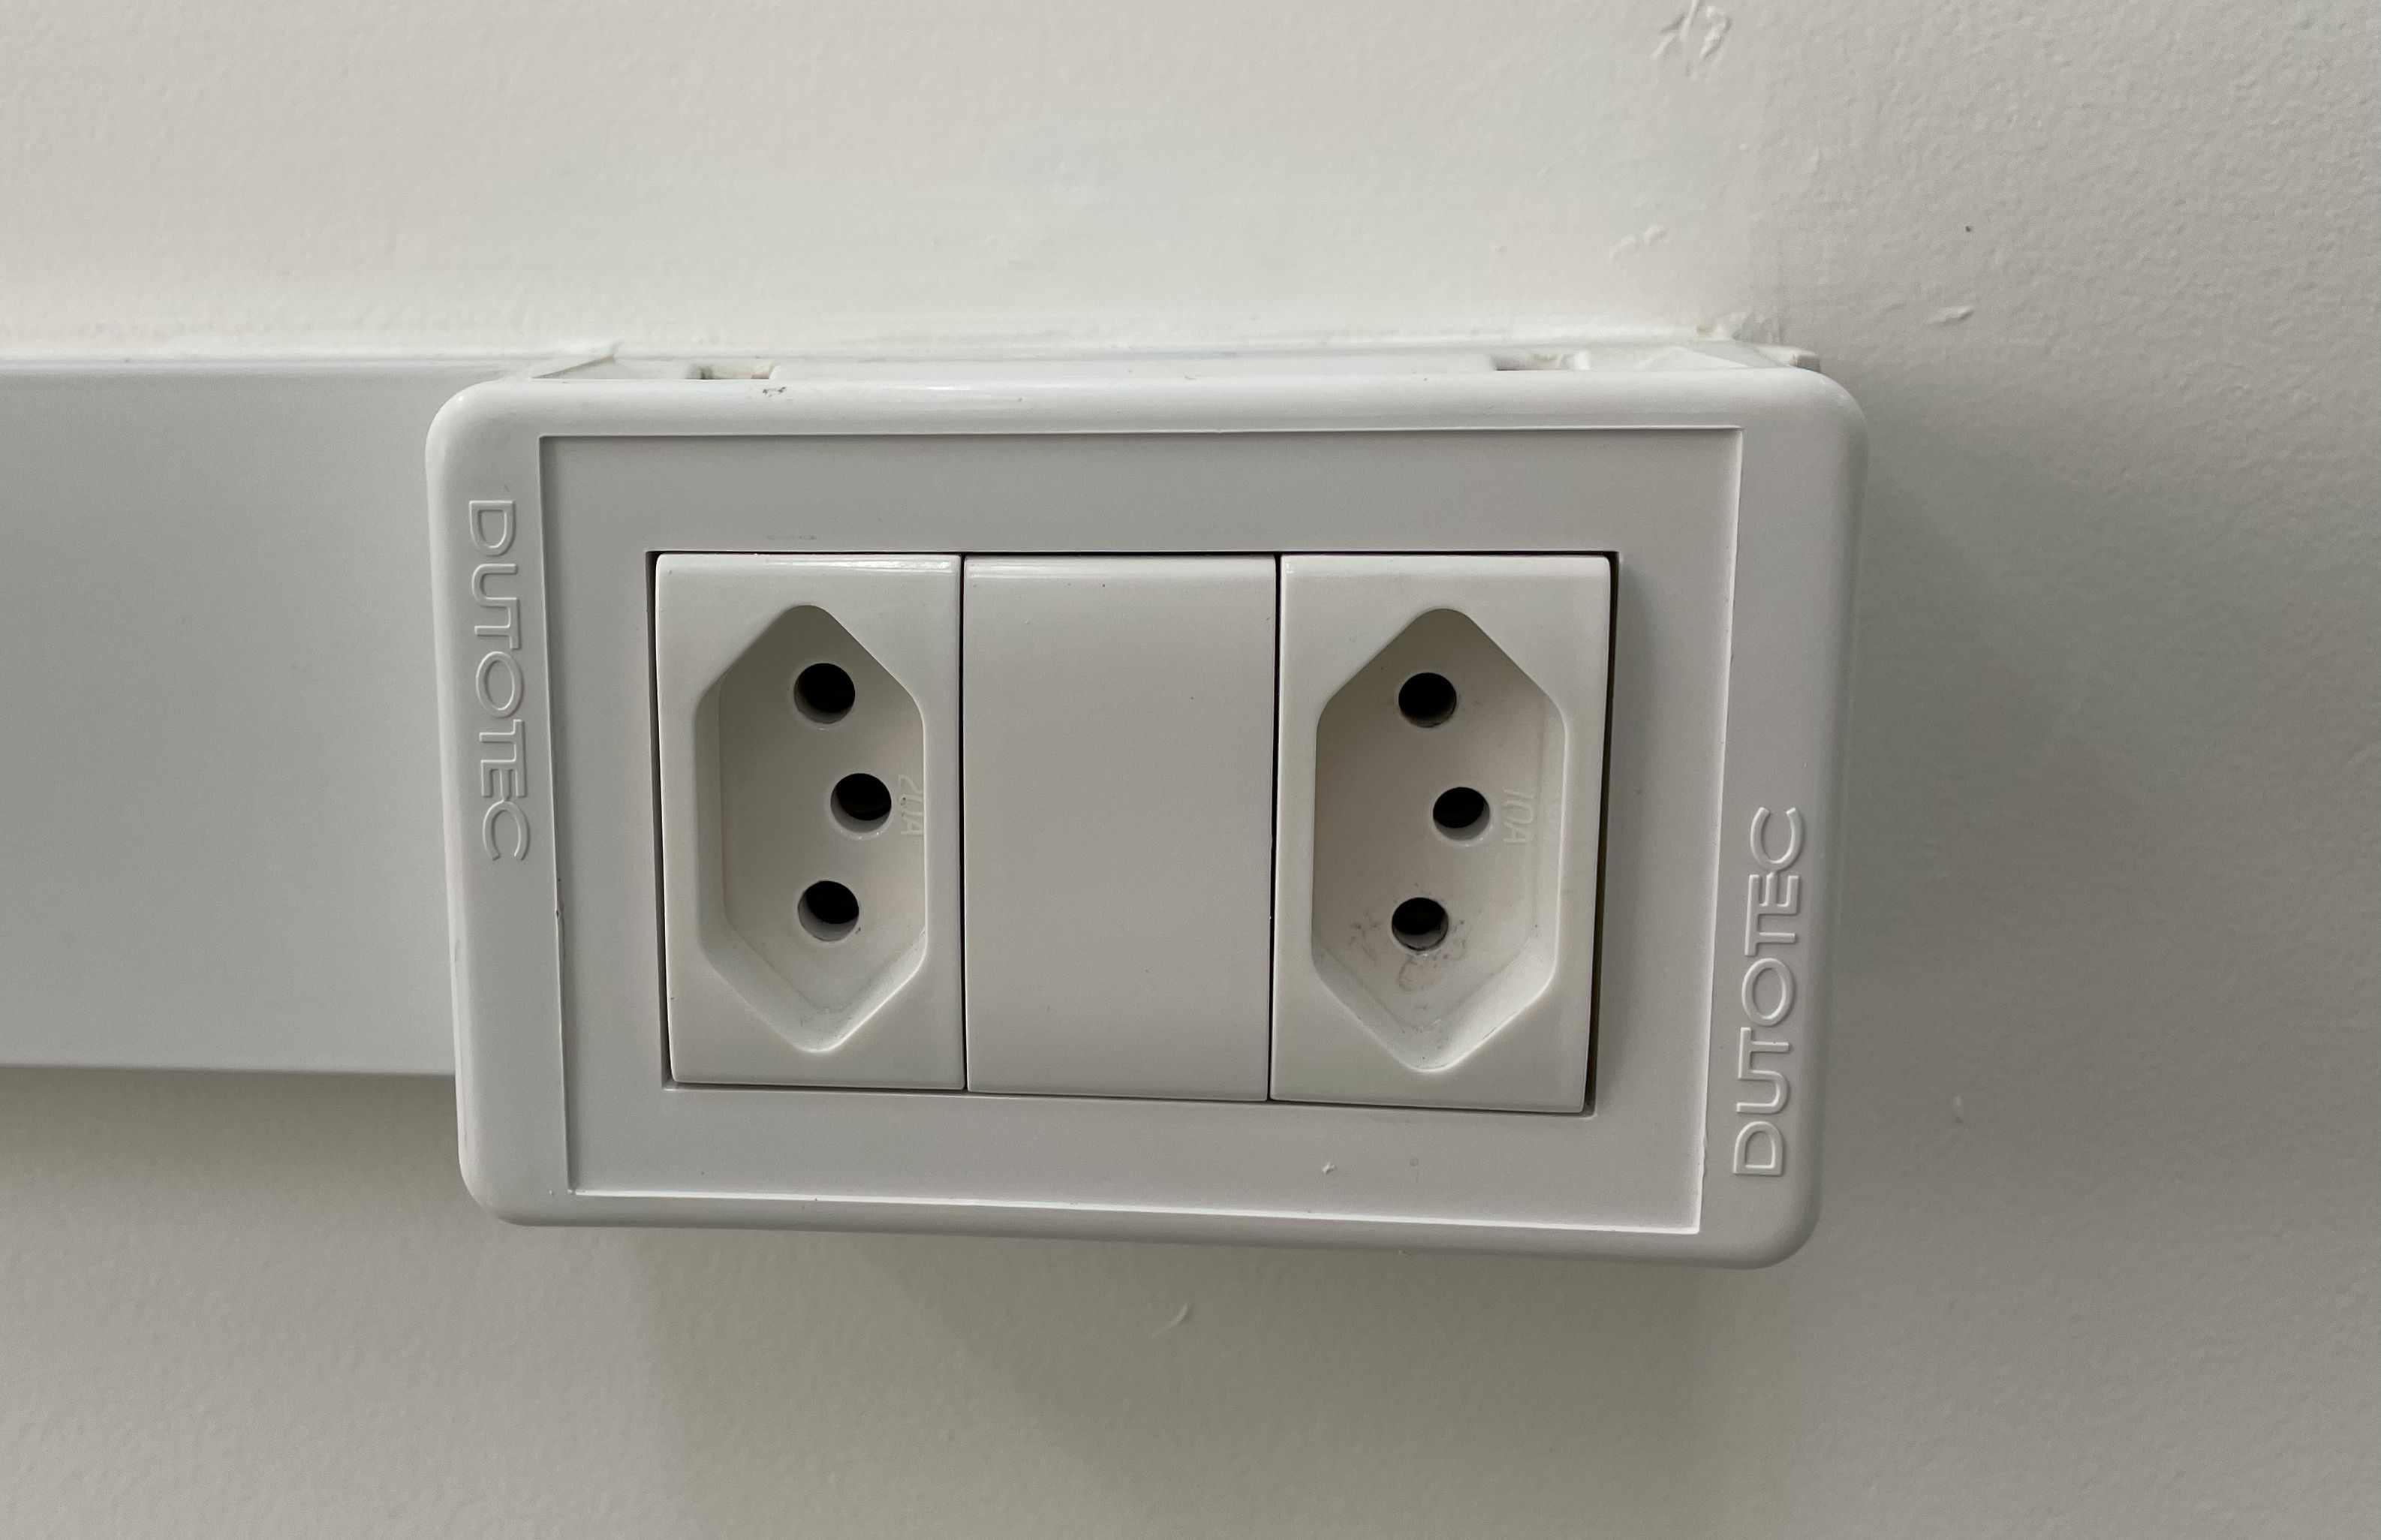
\includegraphics[width=\textwidth]{Figures/4. Socket/tomada2.jpg}
				\caption{Duas tomadas aparentes 127V}
				\label{fig: style 2 image a}
			\end{subfigure}
			\hfill
			\centering
			\begin{subfigure}[b]{0.23\textwidth}
				\centering
				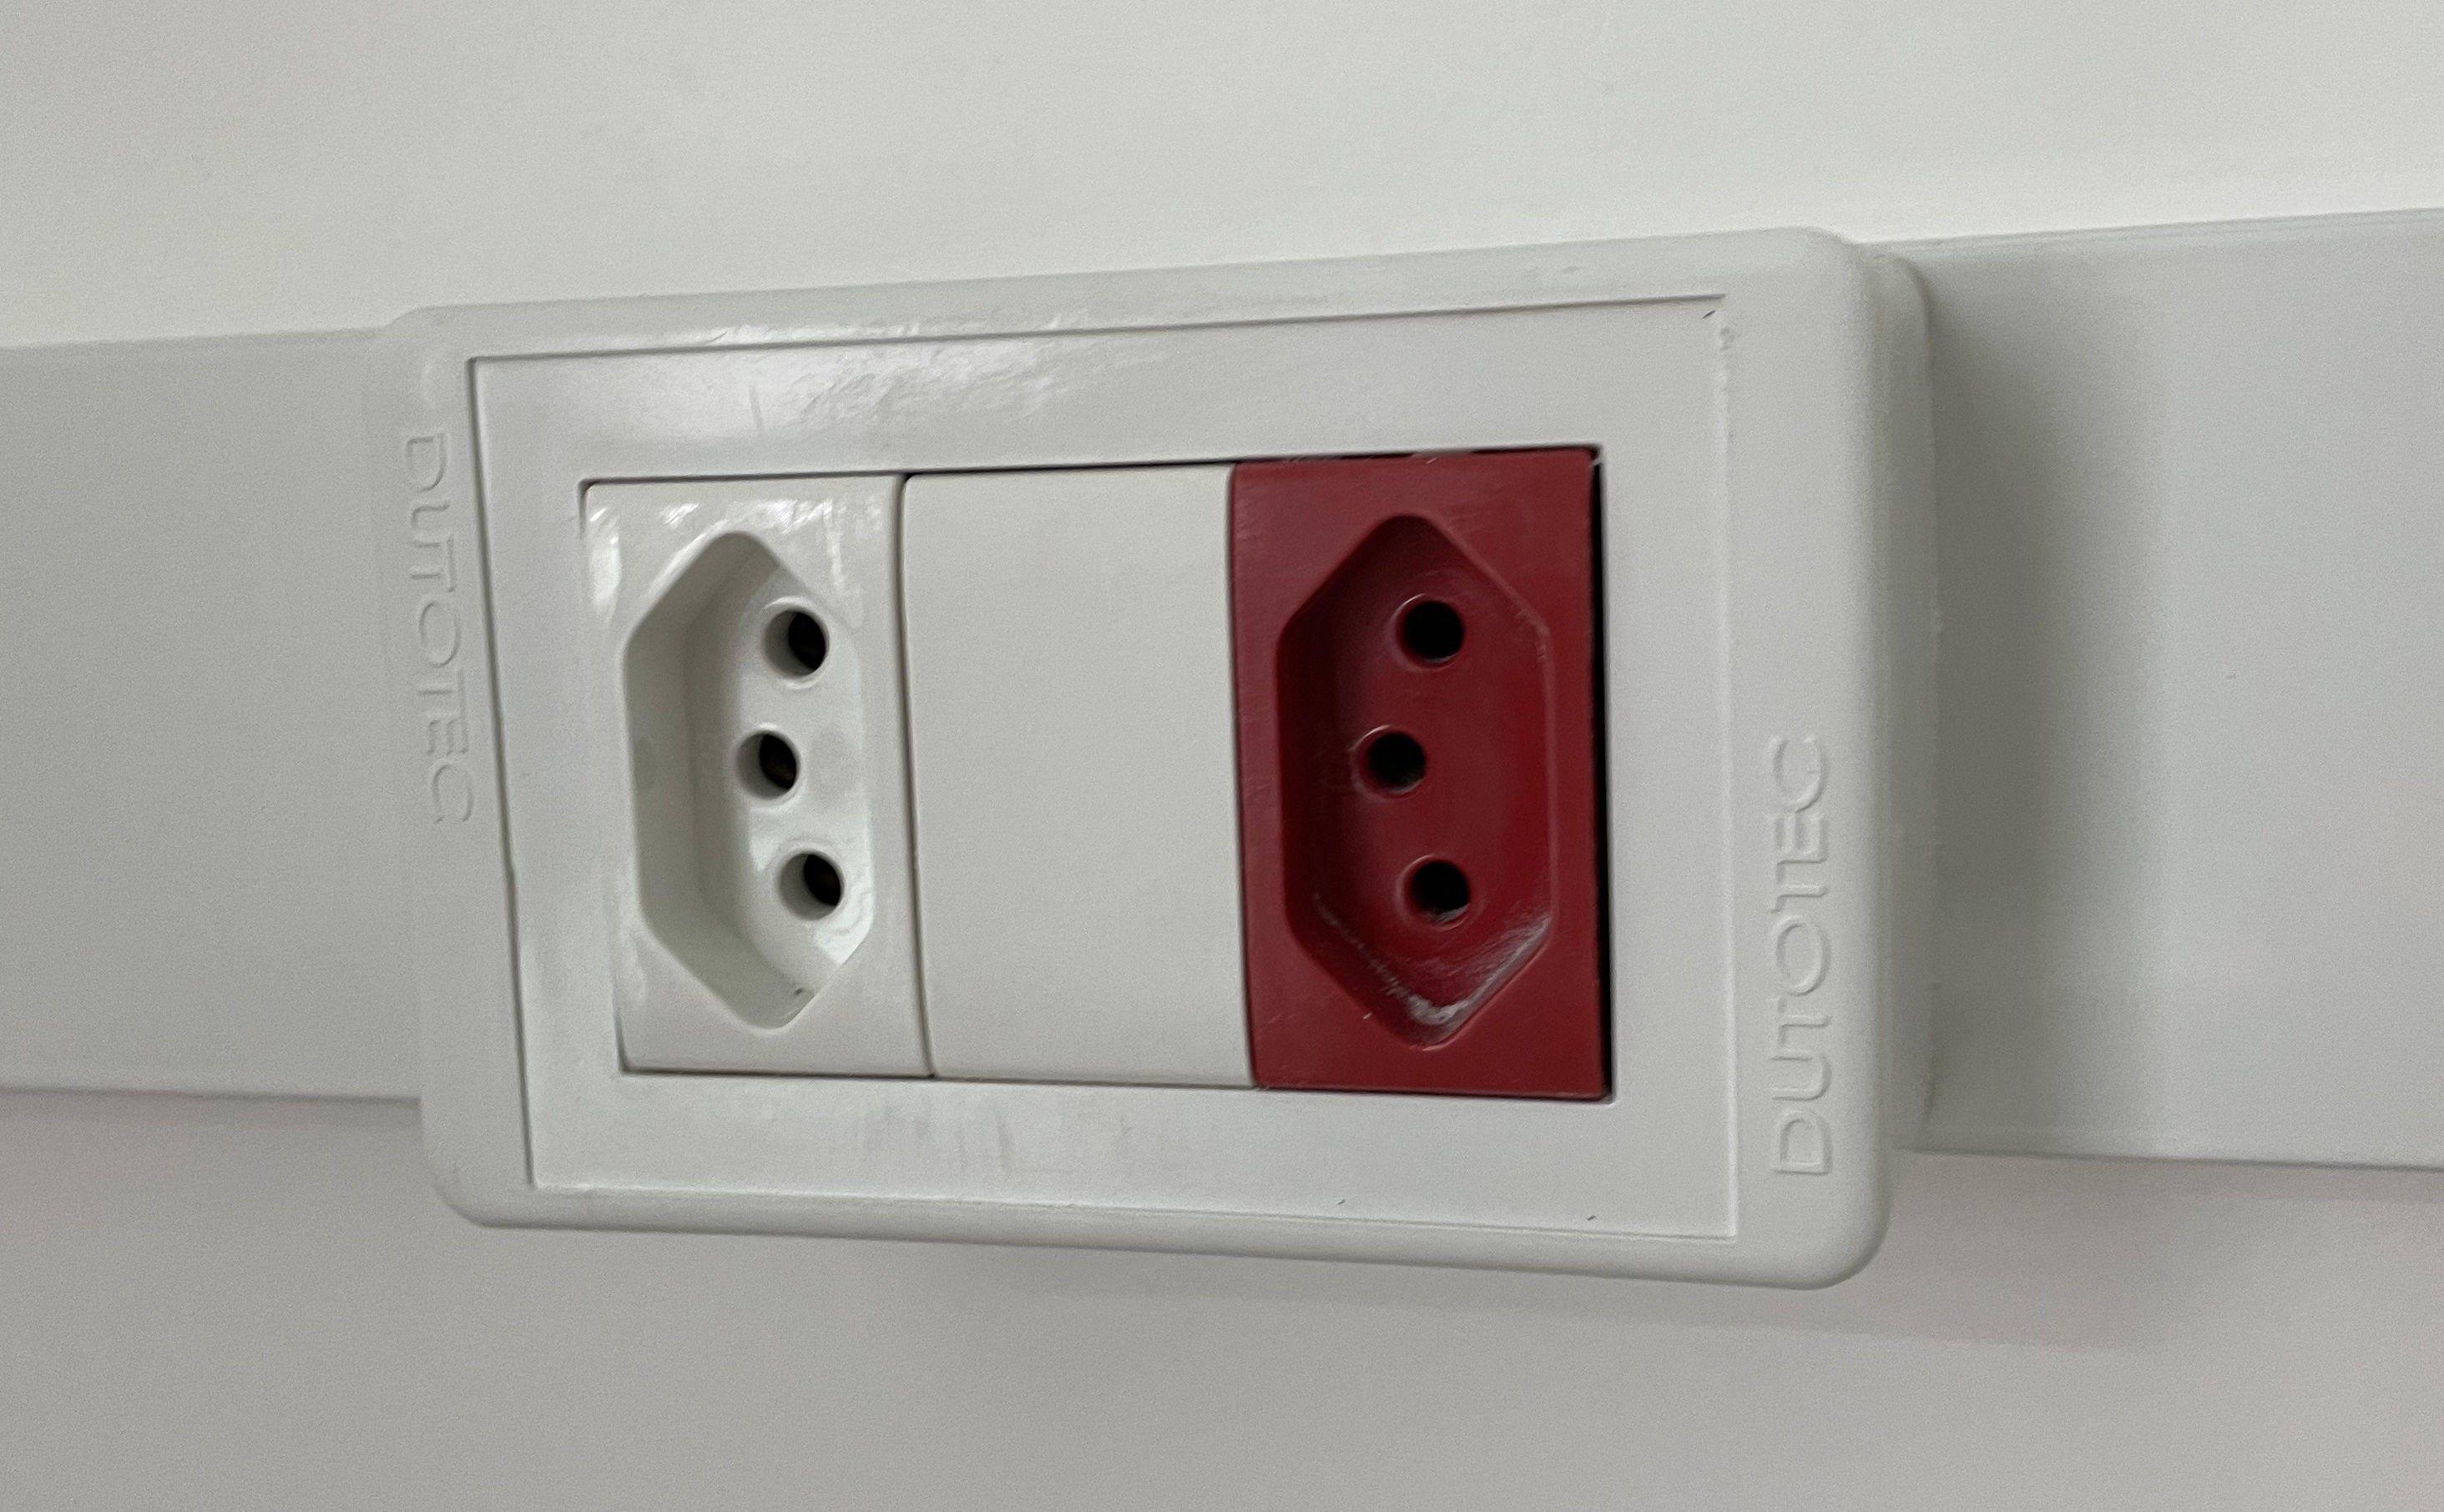
\includegraphics[width=\textwidth]{Figures/4. Socket/tomada3.jpg}
				\caption{Tomadas aparentes 127V e 220V}
				\label{fig: style 2 image b}
			\end{subfigure}
			\hfill
			\begin{subfigure}[b]{0.23\textwidth}
				\centering
				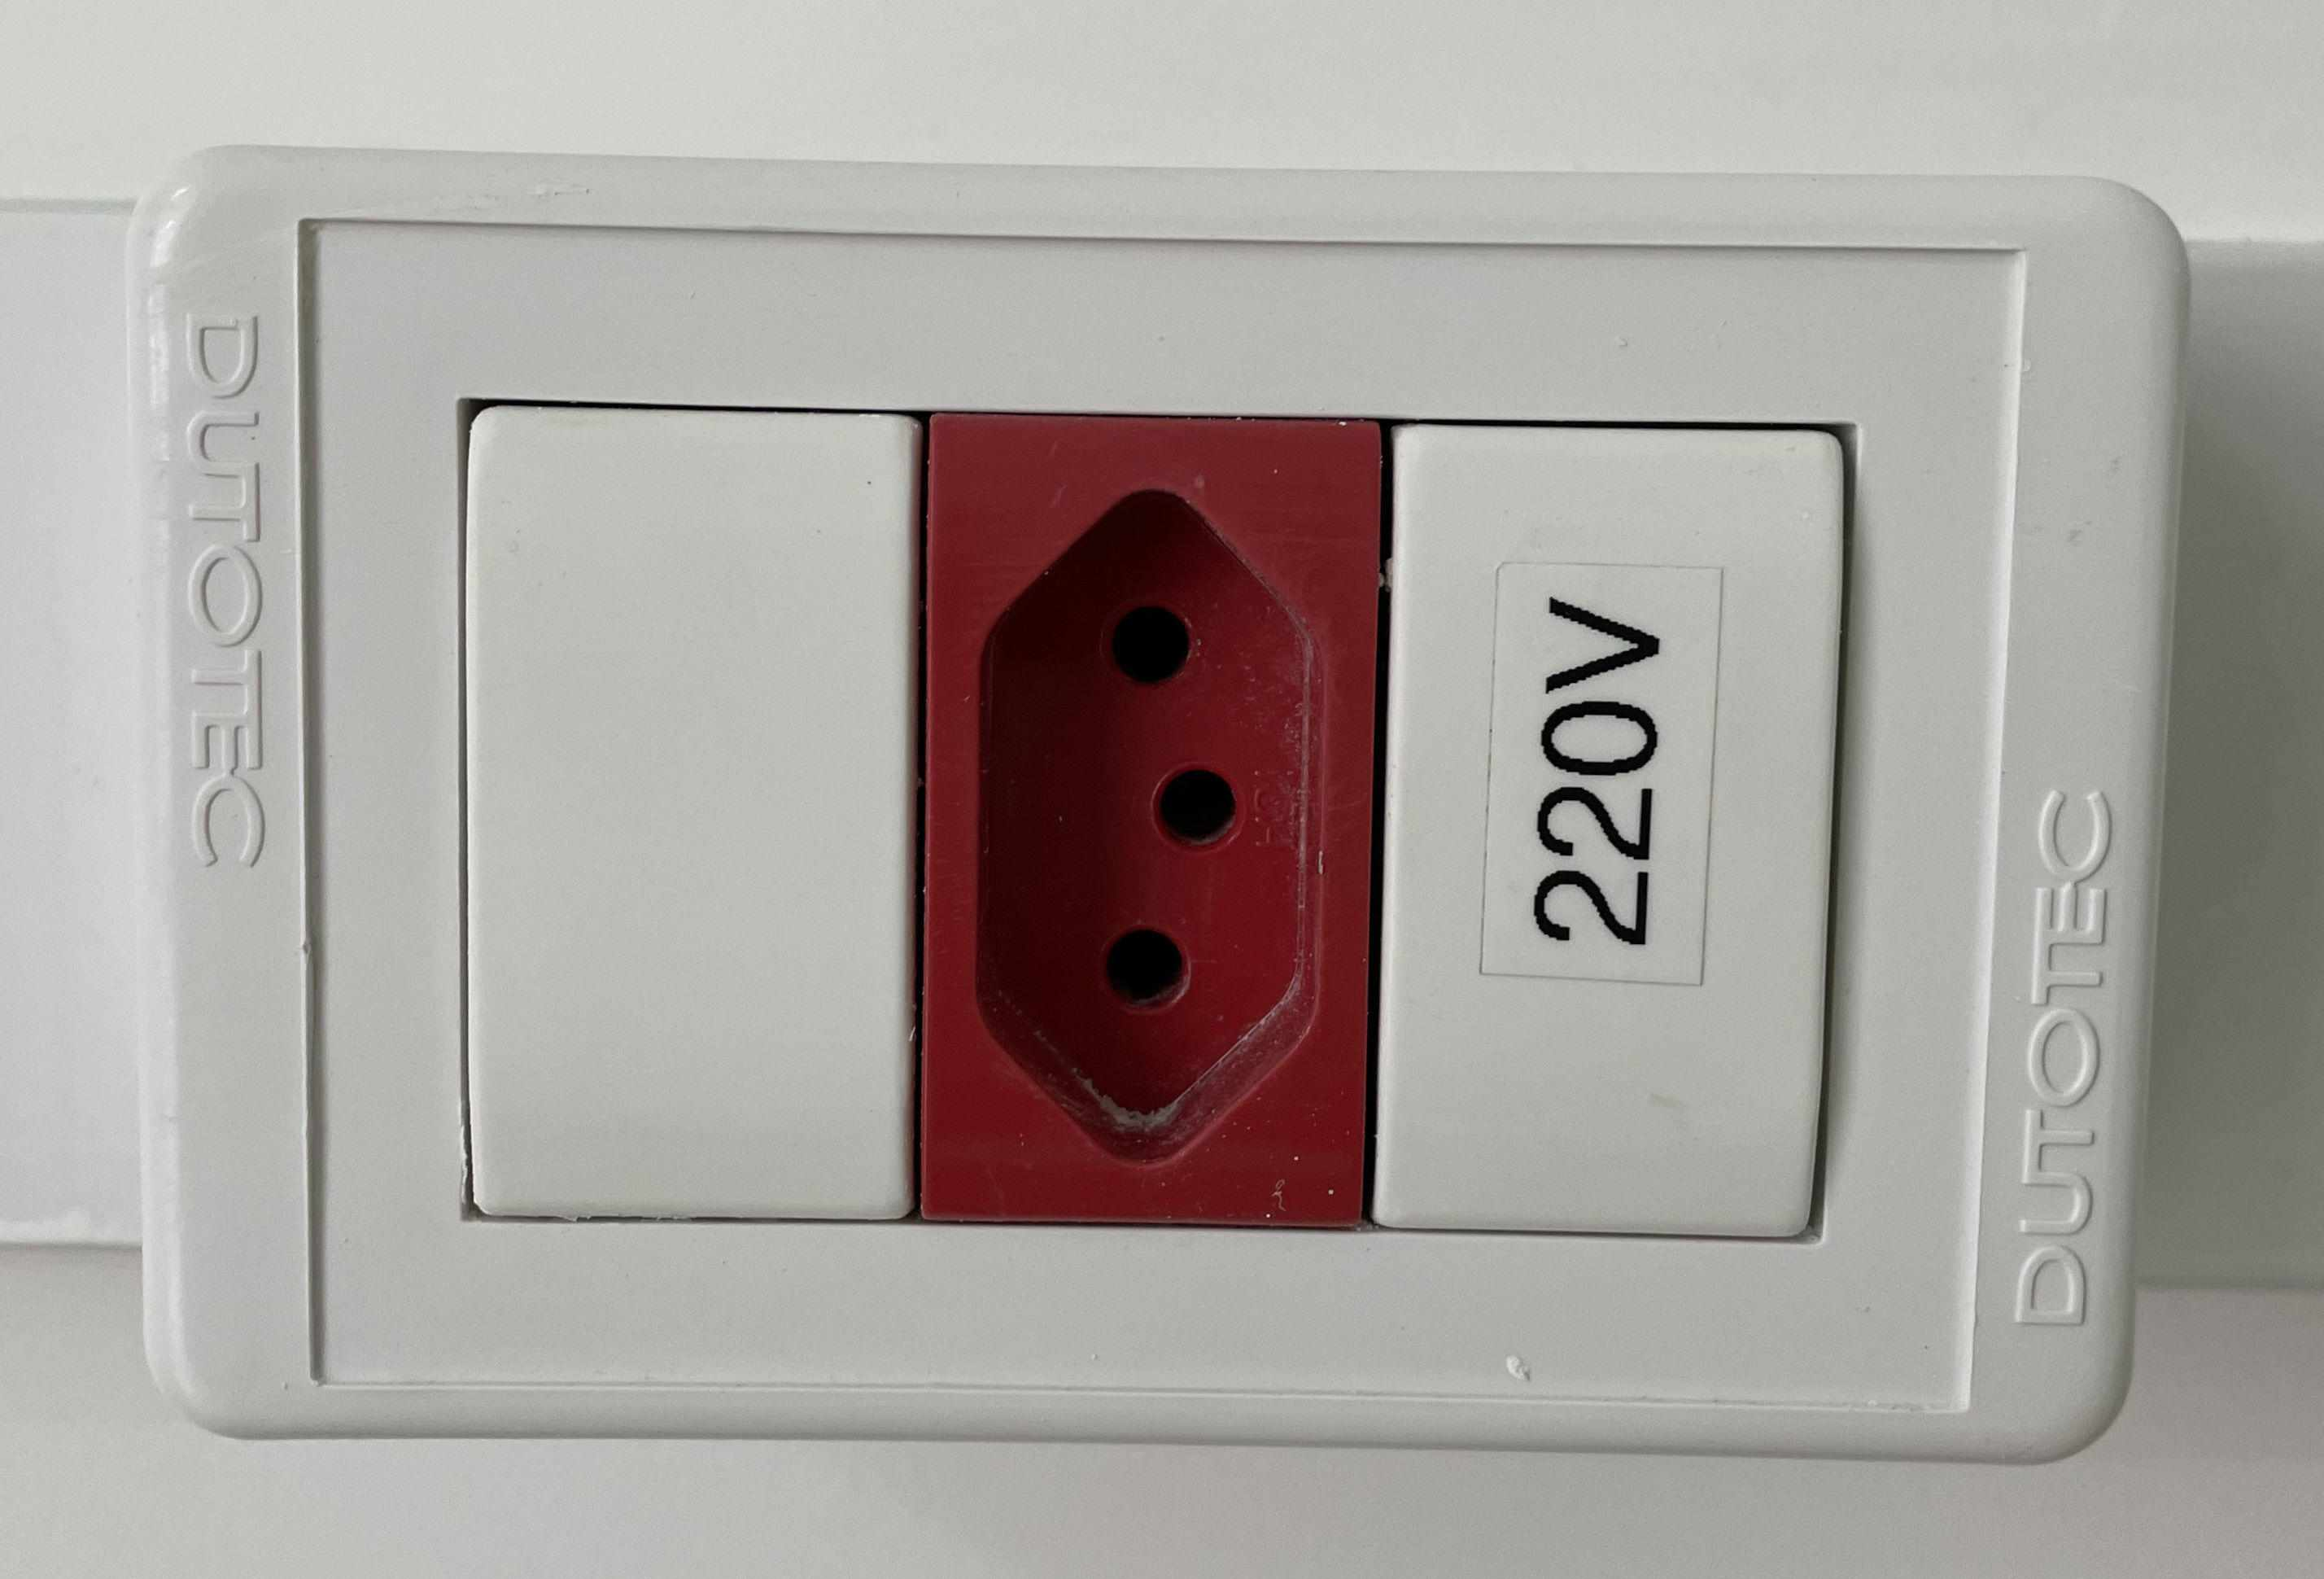
\includegraphics[width=\textwidth]{Figures/4. Socket/tomada4.jpg}
				\caption{Tomada aparente 220V já rotulada}
				\label{fig: style 2 image c}
			\end{subfigure}
			\hfill
			\begin{subfigure}[b]{0.23\textwidth}
				\centering
				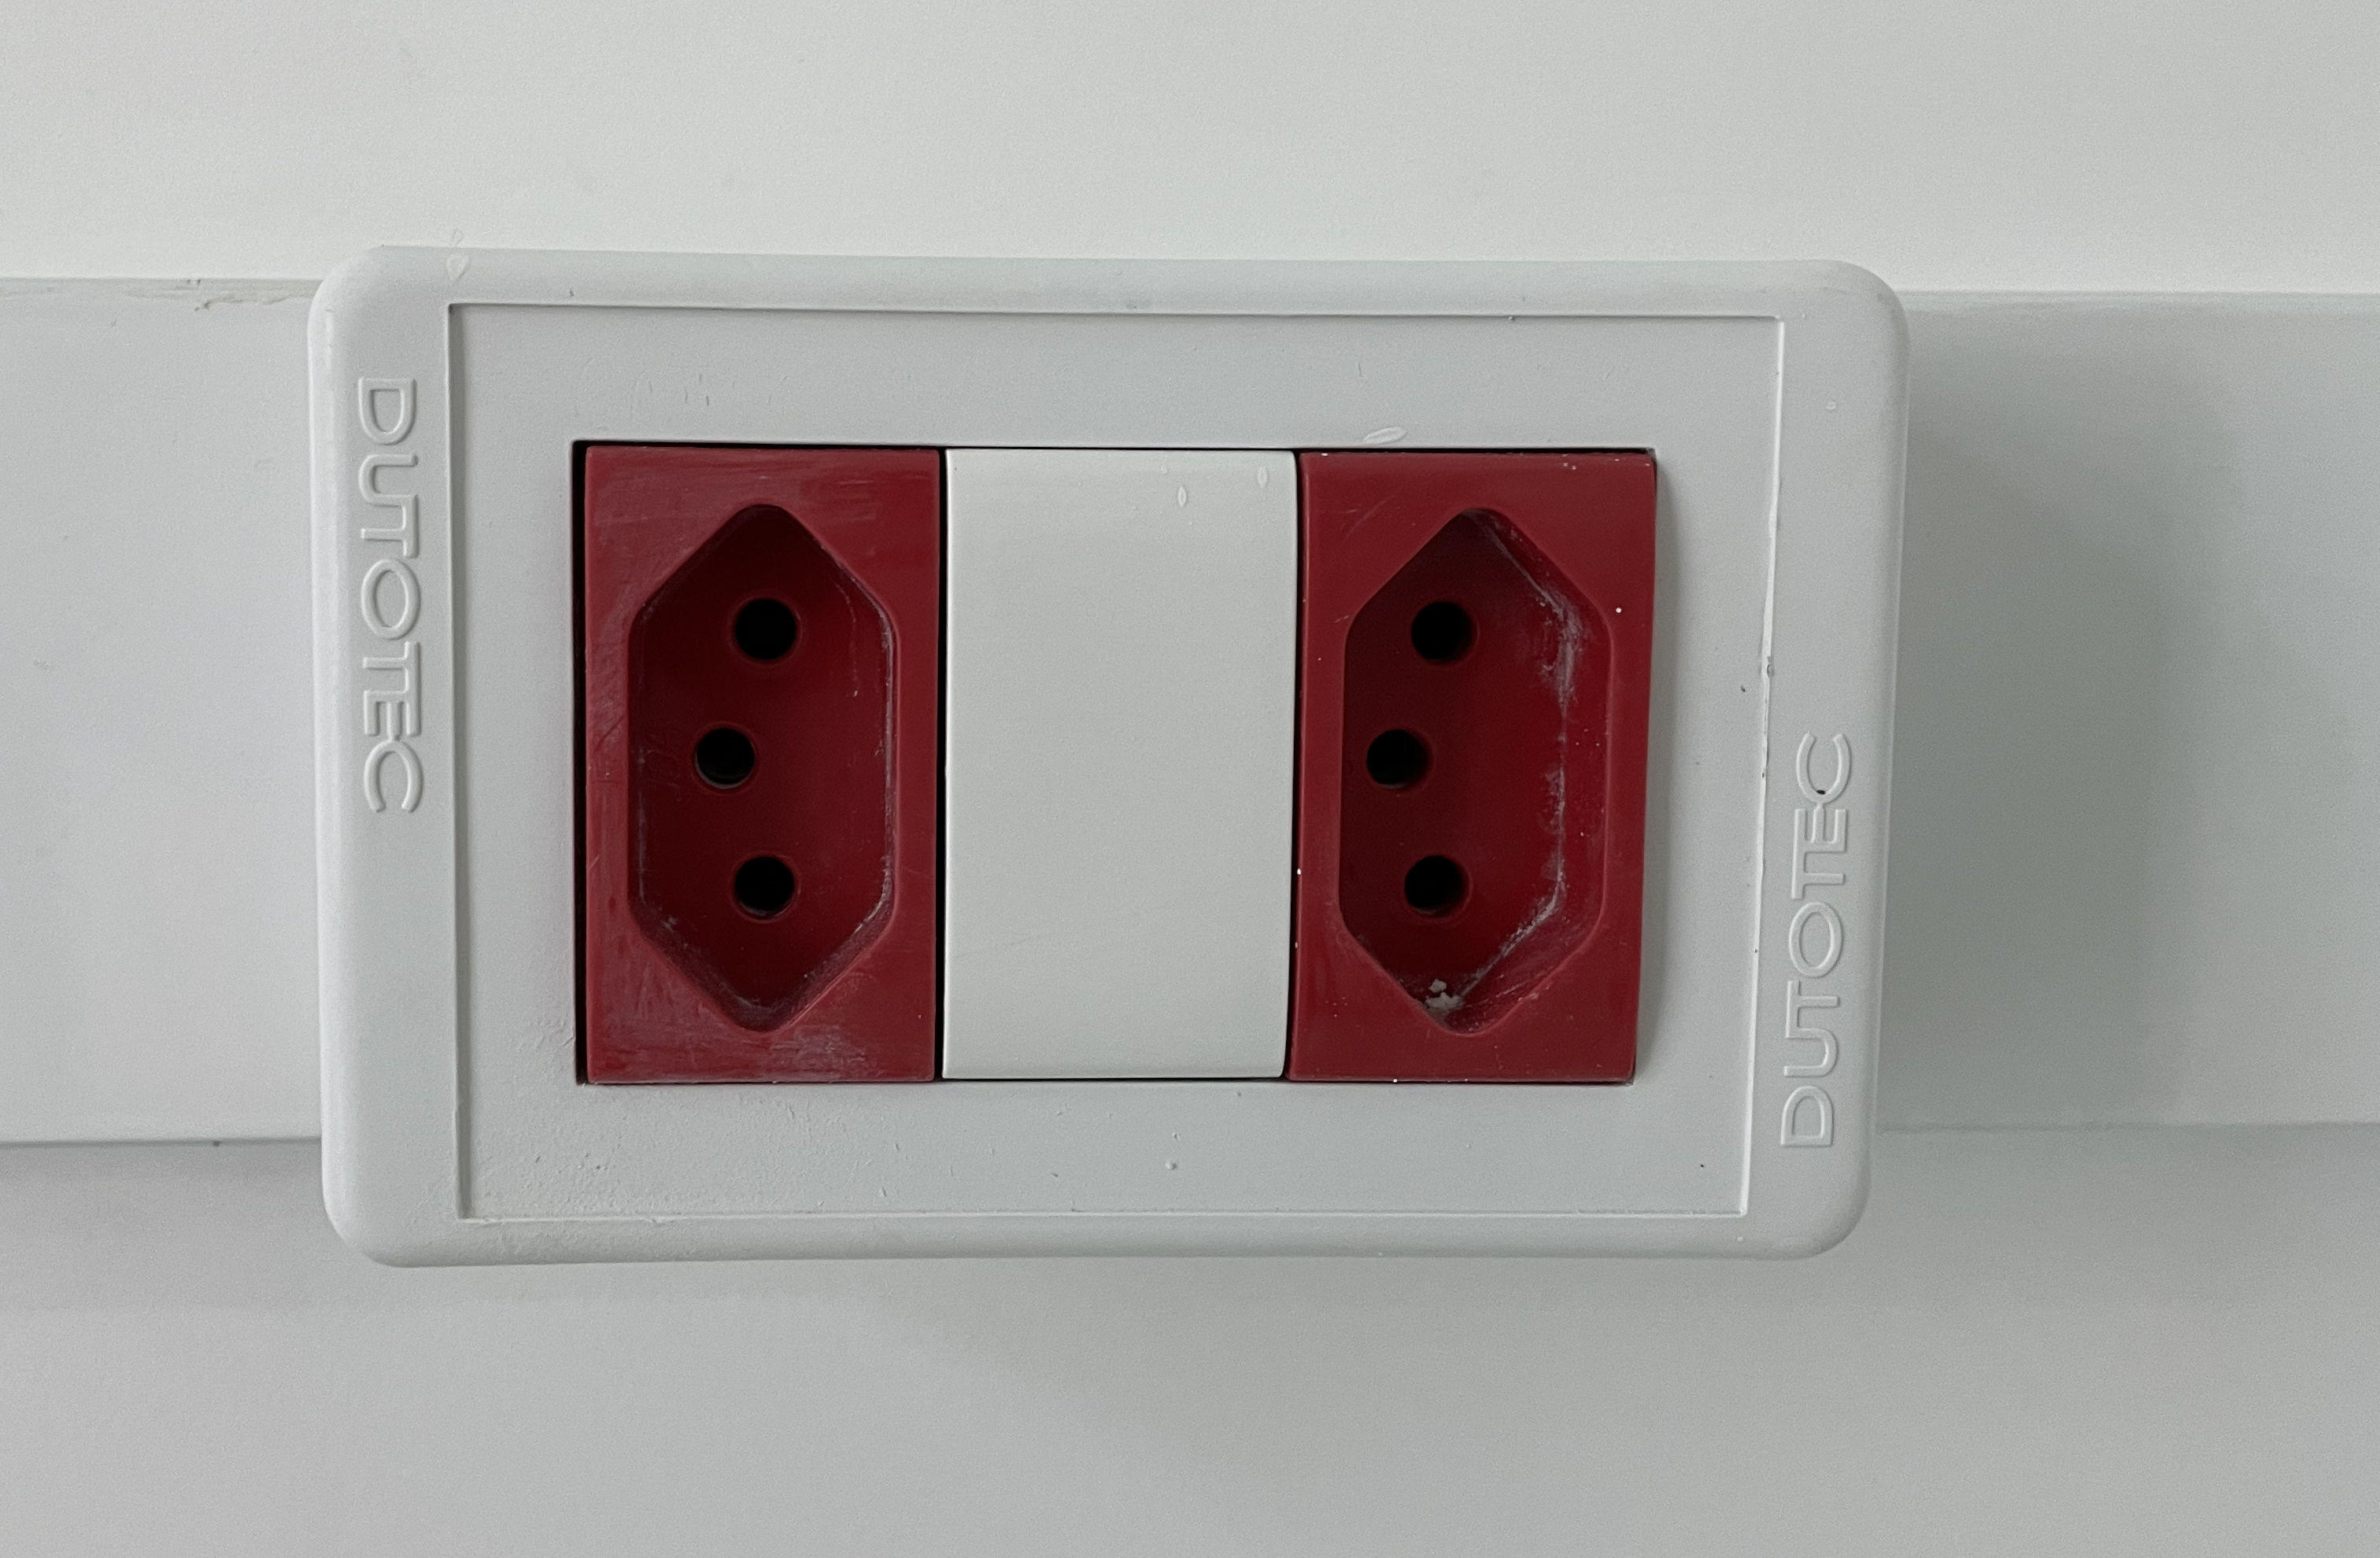
\includegraphics[width=\textwidth]{Figures/4. Socket/tomada5.jpg}
				\caption{Duas tomadas 220V (sem identificação)}
				\label{fig: style 2 image d}
			\end{subfigure}
		\caption{Exemplo de tomadas em roda-meio}
		\label{fig: exemplo-rodameio}
	\end{figure}
	
	\item Existindo um projeto de sistema de segurança e alarme, a alimentação deste sistema deverá originar-se do sistema de energia ininterrupta e, o sistema deverá permanecer em funcionamento mesmo no caso de falta de energia na edificação, ou seja, deverão possuir sistemas de reserva de marcha para até 12 horas de falta total de energia.
	
	\item Ao dimensionar os eletrodutos de tomadas, os mesmos deverão ser dimensionados com diâmetro mínimo de 1"
	
	\item Alguns equipamentos e potências usualmente encontradas durante a fase de coleta de dados (levantamento):
		\begin{table}[ht]
			\rowcolors{2}{Tue-red!10}{white}
			\centering
			\caption{Potências usuais}
			\begin{tabular}[t]{ccc}
				\toprule
				\color{Tue-red}\textbf{Equipamento}&\color{Tue-red}\textbf{Pot. mínima}&\color{Tue-red}\textbf{Pot. máxima}\\
				\midrule
				Capelas&600W&600W\\
				Cabine de segurança biológica&1200W&1200W\\
				Geladeiras "comuns"&150W&300W\\
				Freezers "comuns"&150W&300W\\
				Freezers $<$ -20$^{\circ}$ C&1500W&2400W\\
				Tomadas sem carga específica(administrativo)&200W&200W\\
				Tomadas sem carga específica(laboratório)&200W&300W\\
				\bottomrule
			\end{tabular}
			\label{table: potencias}
		\end{table}

	\begin{figure}[H]
		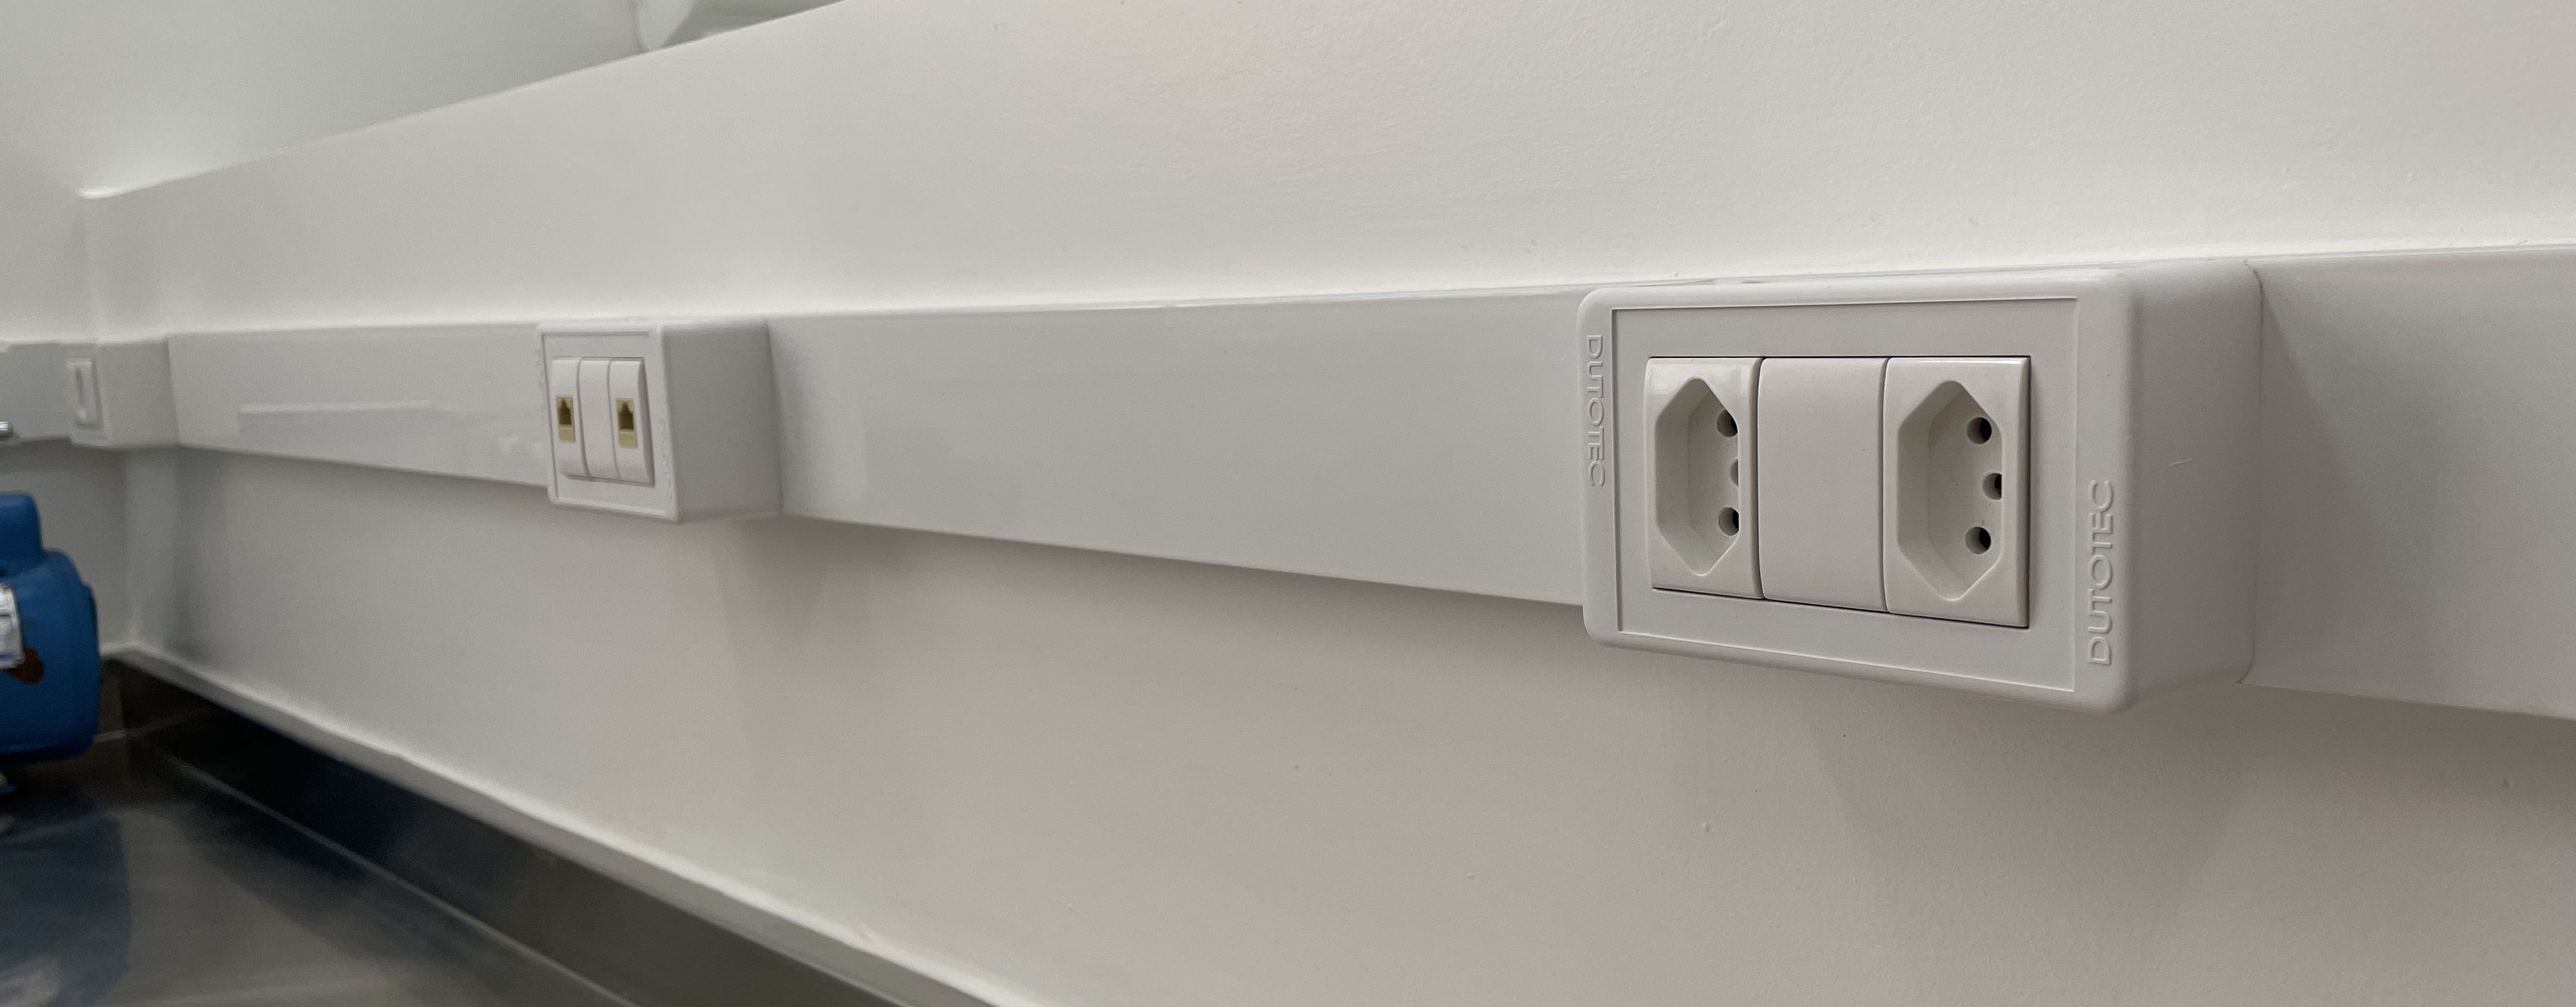
\includegraphics[width=\linewidth]{Figures/4. Socket/tomada1.jpg}
		\caption{Duas tomadas 127V montadas num porta equipamentos}
		\label{fig: tomada rodameio}
	\end{figure}
	\end{enumerate}
